
%%%%%%%%%%%%%%%%%%%%%%%%%%%%%%%%%%%%%%%%%%%%%%%%%%%%%%%%%%%%%%%%%%%%%%%%%%%%%
%% Descr:       Vorlage für Berichte der DHBW-Karlsruhe, Ein Kapitel
%% Author:      Prof. Dr. Jürgen Vollmer, vollmer@dhbw-karlsruhe.de
%% $Id: kapitel2.tex,v 1.5 2017/10/06 14:02:51 vollmer Exp $
%%  -*- coding: utf-8 -*-
%%%%%%%%%%%%%%%%%%%%%%%%%%%%%%%%%%%%%%%%%%%%%%%%%%%%%%%%%%%%%%%%%%%%%%%%%%%%%%%

\chapter{Umsetzung}
\label{chap:Umsetzung}
Dieses Kapitel greift die in der Konzeption (\ref{chap:Konzeption}) aufgeführten Planungen und Ideen auf und legt die Implementierung, bzw. 
Umsetzung detaillierte dar. Darunter sind Lösungsansätze aufgezeigt und aufgetretene Probleme und deren Behebung dokumentiert. Allgemein zählt 
dazu die Umsetzung des Startmenüs und der beiden Kernfunktionen. Sowohl die Frontend- als auch die Backend-Aspekte werden in der Implementierung 
(\ref{chap:implementierung}) aufgezeigt. 

\section{Implementierung}
\label{chap:implementierung}
Aufgrund der zuvor dargelegten Konzeption, ging es an die Umsetzung des Konzepts und an die Implementierung der Funktionen, die das System ausmachen. 
%Nachdem die Konzeption endgültig abgeschlossen war, ging es an die Umsetzung des Konzepts und an die Implementierung der Funktionen, die das System 
%ausmachen. 
\\ 
Die Use Cases und deren Implementierung wurden nach logischer und chronologischer Reihenfolge entwickelt. % und dokumentiert. 
Diese festgelegte Reihenfolge 
ist auch der Abbildung (\ref{pic:anwendungsfall}) zu entnehmen. Angefangen mit dem Startmenü, das dem Nutzer die Möglichkeit offenbart, zwischen den Funktionen 
zu wählen, folgte die Implementierung der Scan-Phase, in der die realen Objekte virtualisiert und im Raum platziert werden. Zuletzt kam die Visualisierungs-Phase, 
welche aufbauend auf die Scan-Phase funktioniert und die zuvor gescannten Objekte erneut virtuell im Raum einsetzt. 
%\\ 
%Beim ersten Gebrauch der Anwendung ist eine vorzeitige Nutzung der Visualisierungs-Phase ohne weiteres nicht möglich. Zuvor muss der Nutzer einen Scan durchführen, sodass 
%das System Daten generiert, Informationen liefert und diese zur Verfügung stellt. Dies hat zur Folge, dass die zweite Kernfunktion mit den zuvor erzeugten Informationen 
%durch die Scan-Phase operiert und ausgeführt werden kann. 
%\\ 
%\linebreak 
%Aufgeteilt wurden die Use Cases der Anwendung jeweils immer nach Frontend und Backend, demnach wird auch die Dokumentation in diesem Stil geschildert. 
\\ 
\linebreak
%Bevor die Umsetzung verwirklicht werden konnte, wurden vorab noch die letzten Vorbereitungen durchgeführt.
%\\ 
Zum Start der eigentlichen Implementierung war es die Aufgabe, die Entwicklungsumgebung zu wählen und einzurichten, um bestmöglich arbeiten zu können. Als 
\ac{IDE} wurde die speziell für Android-Applikationen entwickelte Software \textit{Android Studio} ausgesucht. Diese ist besonders für die Entwicklung von 
Android-Applikation geeignet, ausschließlich für Hardware, dessen Software das Android Betriebssystem nutzt. 
\\
Android Studio ist von Google LLC. und JetBrains entwickelt und basiert auf der IntelliJ IDEA Community Edition \acs{IDE}. Als 
Build-Management-Automatisierungs-Tool stellt Android Studio das Tool Gradle zur Verfügung, welches die zu bauenden Projekte durch die verwendeten 
Dependencies, Frameworks und Tools beschreibt. Um die notwendigen Libraries in der Applikation verwenden zu können, werden in dieser Datei unter 
anderem die Bibliotheken und deren verwendete Version eingetragen. Im Fall des zu entwickelnden Unterstützungssystems wurden dort die Bibliotheken zur 
Nutzung der Android Architecture Components eingetragen, darunter Room und LiveData. 
Darüber hinaus wird dort auch die Version des ARCore Frameworks und des Sceneform \acs{SDK}s verwaltet, welches ebenso essentielle Bestandteile der 
Applikation sind.
\\ 
Nachdem alle Abhängigkeiten erfolgreich eingebunden waren, wurden zur übersichtlichen Gestaltung der Klassen, Objekte, ViewModel, Repositories und Activities 
eine Ordnerstruktur angelegt, die alle Klassen des gleichen Typs im Laufe der Entwicklung beinhalten sollten. Dadurch kann bei der Programmierung besser und 
übersichtlicher durch das Projekt navigiert werden und  es befinden sich alle Klassen ähnlicher Eigenschaften im selben Zielordner. 
\\ 
\linebreak
Damit im Laufe der Entwicklung die Applikation bestmöglich getestet werden konnte, war es notwendig, ein Testgerät zu verwenden. Mit dem verfügbaren 
Emulator\footnote{Ein System, das ein anderes in speziellen Teilbereichen nachbildet} von Android Studio konnte keine realitätsnahe Testung 
durchgeführt werden. Deshalb wurde zum Testen der Anwendung ein Smartphone benutzt.%Dieses musste zu Anfang unter den vorbereitenden Maßnahmen des 
%Projekts organisiert werden.
\\ 
\linebreak
%Nachdem nun alle Schritte abgeschlossen waren, ging es an die Entwicklung des ersten Use Cases, dem Startmenü, um die Grundlage des Systems zu festigen.  
Grundlegend wurden für die Designs der Benutzeroberflächen Prinzipien der \ac{UX}, berücksichtigt. Darunter folgende Punkte: 
%\pagebreak
\begin{itemize}
    \item Übersichtlichkeit (Digestibility): Auf einen Blick verstehen, worum es geht. Der User versteht intuitiv was zu tun ist.
    \item Klarheit (Clarity): Deutliche und verständliche Ausdrucksweise und klar herauszufindenden Nutzen der Funktion, bzw. Anwendung.
    \item Vertrauen (Trust): Gutes Design erlangt Vertrauen. Offenlegung der Aktionen und Hintergründe. 
    \item Begeisterung (Delight): Komplexe Sachverhalte einfach zu lösen. 
\end{itemize} 
\subsection{Startmenü}
Das Startmenü ist die zentrale Anlaufstelle des prototypischen Unterstützungssystems und bildet den Einstiegspunkt in die Interaktionen zwischen Anwender 
und der Applikation, dem Assistenzsystem.
%\\ 
%Nun folgt die Beschreibung der Implementierung des Startmenüs, sowohl des Frontends als auch des Backends.
\subsubsection{Frontend}
%Wird das Unterstützungssystem heruntergeladen, genauer gesagt auf die verwendete Hardware geladen, folgt das Speichern der Anwendung auf dem Gerät. Die Applikation 
%erscheint auf dem Applikationshauptmenü des Smart-Devices und wird dort zur Nutzung zur Verfügung gestellt. 
%\\ 
%Beim Start öffnet sich das Hauptfenster der Applikation und darin das Startmenü, auf das im Verlauf noch genauer eingegangen wird. 
%\\ 
Zuallererst werden bei initialer Instandsetzung bestimmte Genehmigungen eingeholt, um die Anwendung überhaupt starten zu können. Darunter soll der Nutzer dem System 
die Erlaubnis erteilen, auf die Kamera zugreifen zu dürfen, um die Umgebung in der Hauptfunktion scannen zu können. % muss diese in weiterer Abfolge des Assistenzsystems genutzt werden können. 
Diese Abfrage erfolgt über ein kleines PopUp-Fenster, welches von Android fest vorgegeben ist. %Dieses Fenster ist der Abbildung (\ref{pic:camera_perm}) 
%zu entnehmen. 
Mit dem Zulassen des Zugriffs auf die Kamera kann der Nutzer und die Applikation wie gewünscht fortfahren. %Wird allerdings der Zugriff abgelehnt, kann 
%die Applikation nicht starten, bzw. wird der Zugriff auf die Kamera verweigert, kann die Applikation nicht einwandfrei benutzt werden.     
%\begin{figure}[hbt!]
%    \centering
%    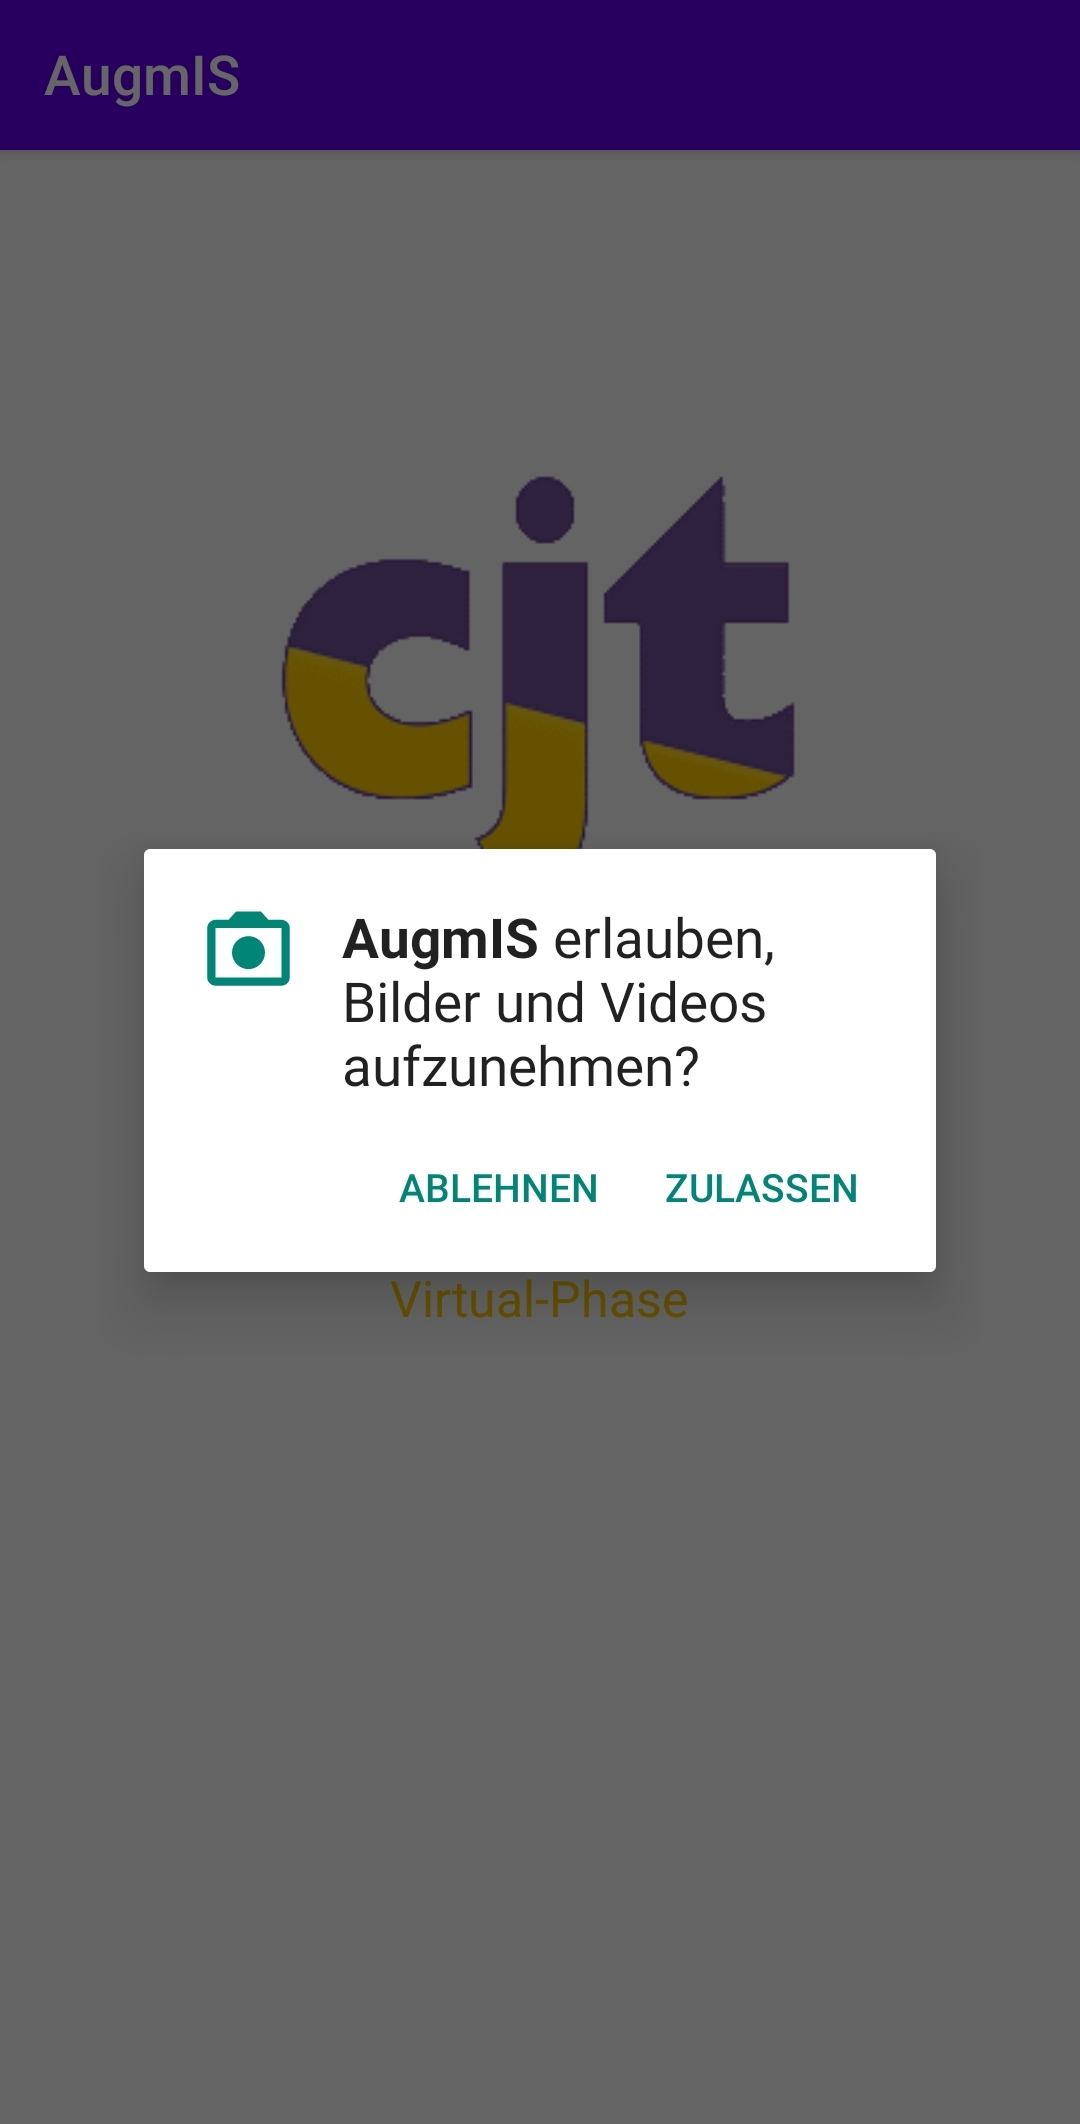
\includegraphics[width=10cm,height=7.5cm,keepaspectratio]{4Umsetzung/Bilder/camera_permission.jpg}
%    \caption{Start der Applikation}
%    \label{pic:camera_perm}
%\end{figure}
\\ 
\linebreak
Da speziell das Assistenzsystem auf die gegebenen Komponenten der Hardware zugreift, z. B. die im Smart-Device integrierte Kamera, zählt diese zu den nativen Applikationen. 
Darunter sind Anwendungen zu verstehen, die ausdrücklich für das Betriebssystem des Endgeräts konzipiert sind oder die zum Beispiel auf die vom Endgerät vorhandenen 
Komponenten zugreifen, wie in etwa auf die Bild-Mediathek, sämtliche Datei-Strukturen oder die oben bereits erwähnte Kamera-Komponente.
\\ 
\linebreak
Angenommen der Nutzer lässt den Zugriff auf die Kamera für das Assistenzsystem zu, dann startet die Applikation wie erwünscht. Darauffolgend ist dann 
das eigentliche Startmenü zu sehen. Diese Ansicht ist der nachfolgenden Abbildung (\ref{pic:startmenu}) zu entnehmen. Die Benutzeroberfläche weist ein sehr einfaches und 
schlicht gehaltenes Design auf. 
Darauf ist das Firmen-Logo der cjt Systemsoftware AG zentriert zu sehen, außerdem zwei farblich voneinander getrennten Buttons zur Navigation innerhalb der Applikation. 
Die Buttons adressieren jeweils die nachfolgende, zugehörige Funktion. Dies sind zum einen der lilafarbene Button, der zur Scan-Phase weiterleitet und zum anderen der 
gelbfarbene Button, der den Nutzer zur Visualisierungs-Phase navigiert. %In der Gesamtheit ist das Layout an den Farben des Firmen-Logos angelehnt und bildet einen 
%ruhigen und harmonischen Einstieg in das Programm. 
\begin{figure}[hbt!]
    \centering
    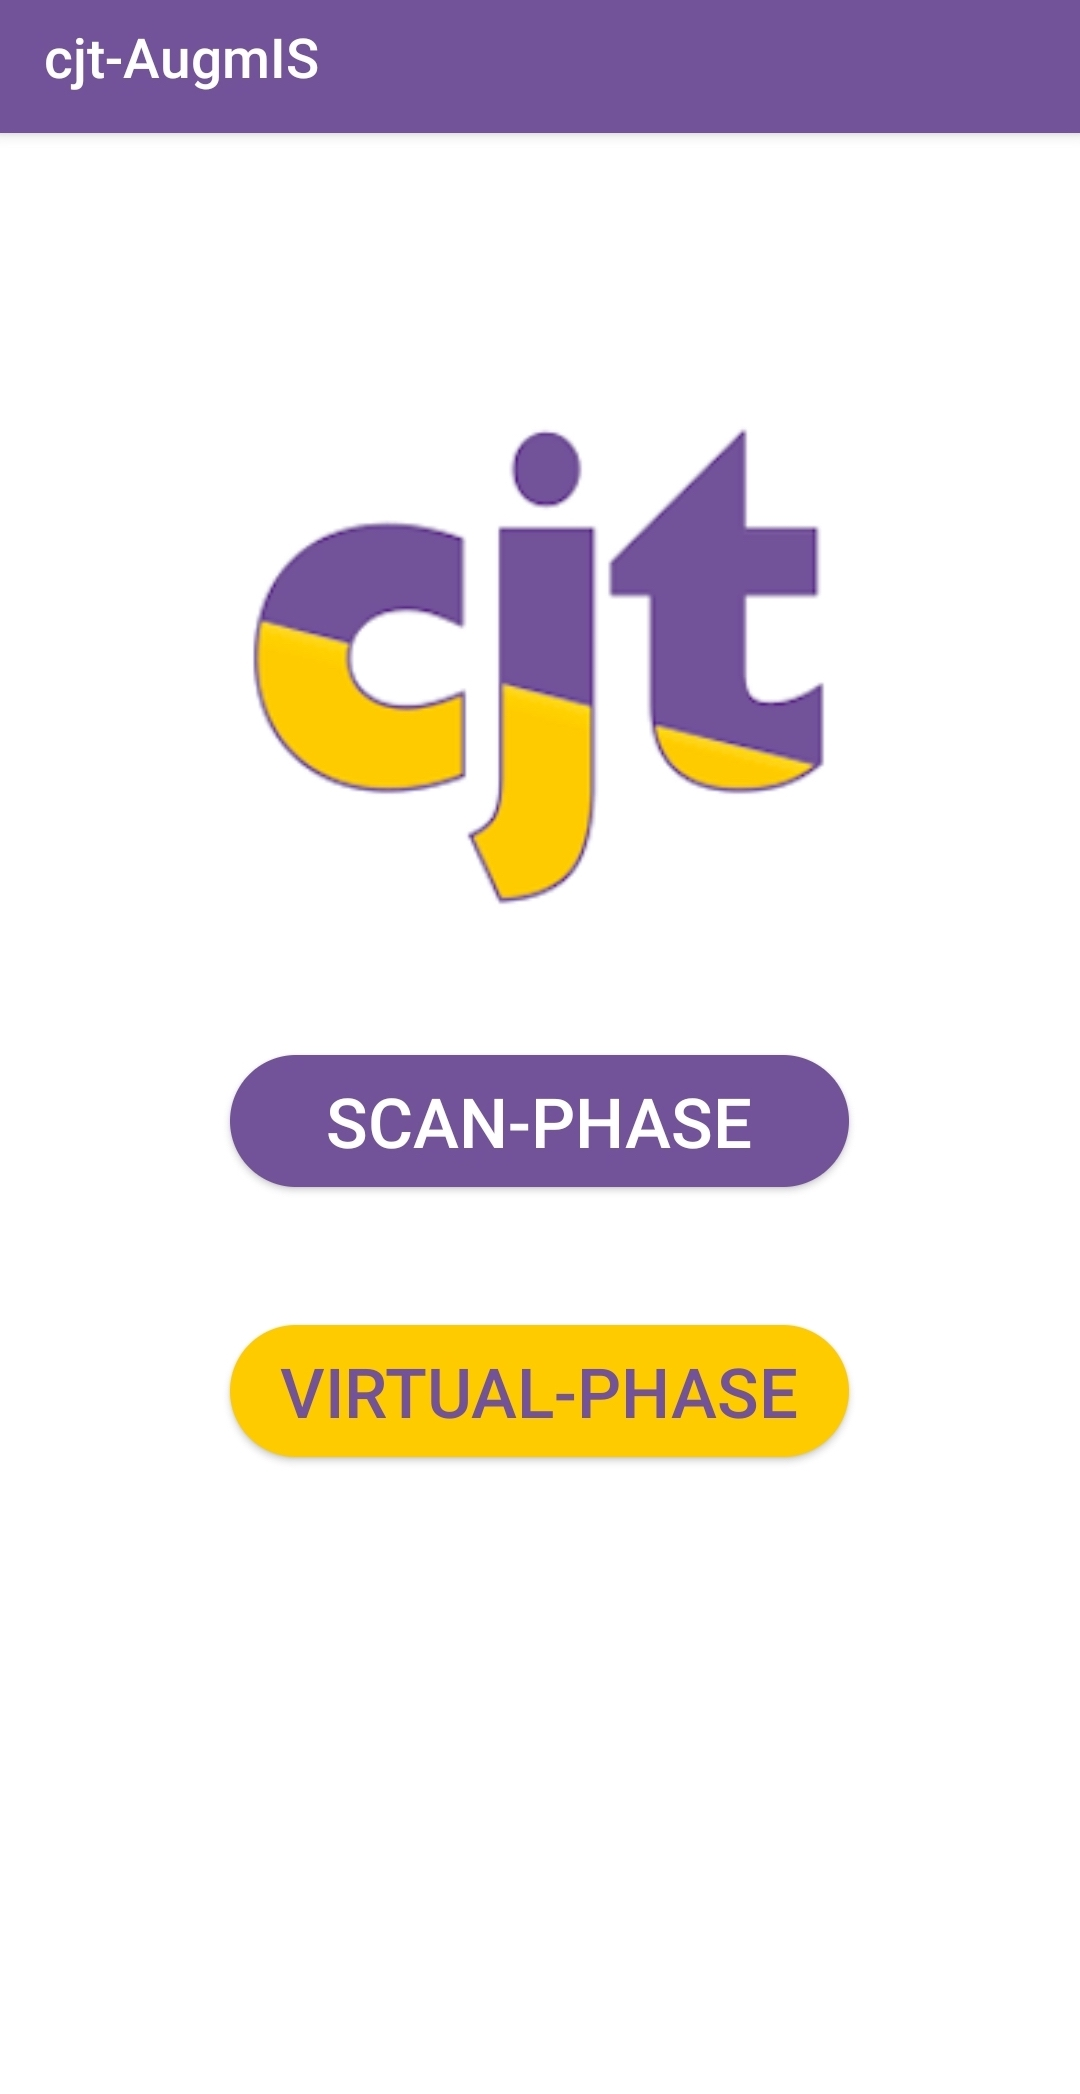
\includegraphics[width=7cm,height=7cm,keepaspectratio]{4Umsetzung/Bilder/startmenu.jpg}
    \caption{Startmenü der Applikation}
    \label{pic:startmenu}
\end{figure}
\\
Die Button-Interaktionen und die jeweils dahinterliegenden Funktionen sind durch den folgenden Programmablaufplan verdeutlicht. 
\begin{figure}[hbt!]
    \centering
    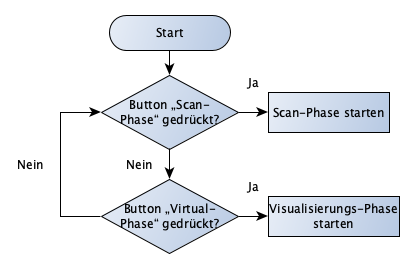
\includegraphics[width=6cm,height=7cm,keepaspectratio]{4Umsetzung/Bilder/startPAP.png}
    \caption{Programmablaufplan des Startmenüs}
    \label{pic:startmenu}
\end{figure}
%\linebreak
%Grundlegend wurden für die Designs der Benutzeroberflächen Prinzipien der \ac{UX}, berücksichtigt. Darunter folgende Punkte: 
%\pagebreak
%\begin{itemize}
%    \item Übersichtlichkeit (Digestibility): Auf einen Blick verstehen, worum es geht. Der User versteht intuitiv was zu tun ist.
%    \item Klarheit (Clarity): Deutliche und verständliche Ausdrucksweise und klar herauszufindenden Nutzen der Funktion, bzw. Anwendung.
%    \item Vertrauen (Trust): Gutes Design erlangt Vertrauen. Offenlegung der Aktionen und Hintergründe. 
%    \item Begeisterung (Delight): Komplexe Sachverhalte einfach zu lösen. 
%\end{itemize} 
%Nachdem das Design des Startmenüs und dem PopUp-Fenster abgeschlossen war, ging es darum, die Funktionalität der UI-Komponenten zu implementieren. 
\subsubsection{Backend}
Durch die schlichte und einfach gehaltene Modellierung des Startmenüs, zählt dieses als Ansicht zum Einstieg in die Nutzung des Assistenzsystems, zur Abfrage der 
\textit{„Camera-Permission“} und zur weiteren Navigation innerhalb der Anwendung.
\\ 
Mit der \textit{„Permission-Request“} wird abgefragt, ob die Genehmigung zur Nutzung der Kamera in der \textit{„AndroidManifest.xml“}-Datei erteilt wurde, bzw. 
dadurch wird das PopUp-Fenster zur Nachfrage der Genehmigung geöffnet und die daraus resultierende Antwort in die Manifest-Datei eingetragen. 
\\ 
\linebreak
Die Manifest-Datei beinhaltet alle optionalen Metadaten, die für das Assistenzsystem benötigt werden. Dazu gehören die Google ARCore-Metadaten, sowie 
grundlegende Informationen über das Projekt, die das Android-System erfordert, um die Applikation installieren und ausführen zu können. Des Weiteren wird 
die Berechtigung zur Kameranutzung benötigt. Ebenso werden Angaben zu Activities, bzw. Benutzeroberflächen gemacht und Stammdaten, z.B. Titel, -bild und 
App-Icon, die das Projekt eindeutig spezifizieren, definiert.
\\ 
\linebreak
Demnach beinhaltet die Backend-Funktion des Startmenüs die Abfrage der \textit{„Camera-Permission“} und die Button-Klick-Funktionen, die den Nutzer 
jeweils auf die von ihm gewählte Funktion weiterleiten. Sozusagen handelt es sich um eine simple Navigation.
%\\ 
%\linebreak
%Als das Startmenü implementiert war, ging es an die Entwicklung der Scan-Phase, der ersten Kernfunktion des Assistenzsystems.

\subsection{Scan-Phase} %Umgebungserkennung /
\label{chap:scan_implementation}
%Bei der Implementierung der Scan-Phase kam es zu den ersten praktischen Berührpunkten mit der Google ARCore \acs{API}. Diese wurde zu Beginn studiert, 
%um einen Überblick, wie die Struktur dieser Schnittstelle aufgebaut ist, zu erlangen. Dadurch konnten Methoden und Funktionen analysiert werden, um im 
%weiteren Verlauf der Entwicklung damit arbeiten zu können.
%\\ 
Die Idee hinter der Scan-Phase ist die Implementierung einer Methode, die es ermöglicht, das Umfeld über die Kamera wahrzunehmen und mit den gewonnenen 
Erkenntnissen über den Raum weiterarbeiten zu können. Die nachstehende Funktion, virtuelle Objekte auf Basis der vom Scan erfahrenen Kenntnissen in 
der Räumlichkeit zu platzieren, arbeitet mit diesen in Erfahrung gebrachten Kenntnisse. 
\\ 
Zur Schaffung einer Grundlage, um die wichtigsten Funktionen zu implementieren, wurden zuallererst die Benutzeroberflächen erstellt. Diese dienen 
unter anderem dazu, den Fokus für die Funktionsweise der eigentlichen Methode nicht zu verlieren. Demnach werden die entwickelten \acs{GUI}s nun aufgeführt 
und näher beschrieben, um Methoden des Backends im Anschluss besser nachvollziehen zu können.
\subsubsection{Frontend}
Das Assistenzsystem verfügt über eine Vollbildkamera-Ansicht, die mit einem weißen Rahmen überlagert ist. Damit können über die Kamera Bilder zentriert 
eingefangen werden. Somit weiß der Nutzer, wie er das Smart-Device in Position bringen muss, damit er das zu scannende Bild über die Kamera 
bestmöglich erfassen kann. 
\\ 
\linebreak
Ursprünglich war die Applikation nicht mit diesem Layout der Abbildung (\ref{pic:image_tracking}) konzipiert, da während der Implementierung der Scan-Phase eine 
schwerwiegende Änderung vorgenommen werden musste. Diese wird in dem Abschnitt der Scan-Phasen-Backend-Entwicklung zu gegebenem Zeitpunkt 
aufgegriffen und genauestens dargelegt. 
\begin{figure}[hbt!]
    \centering
    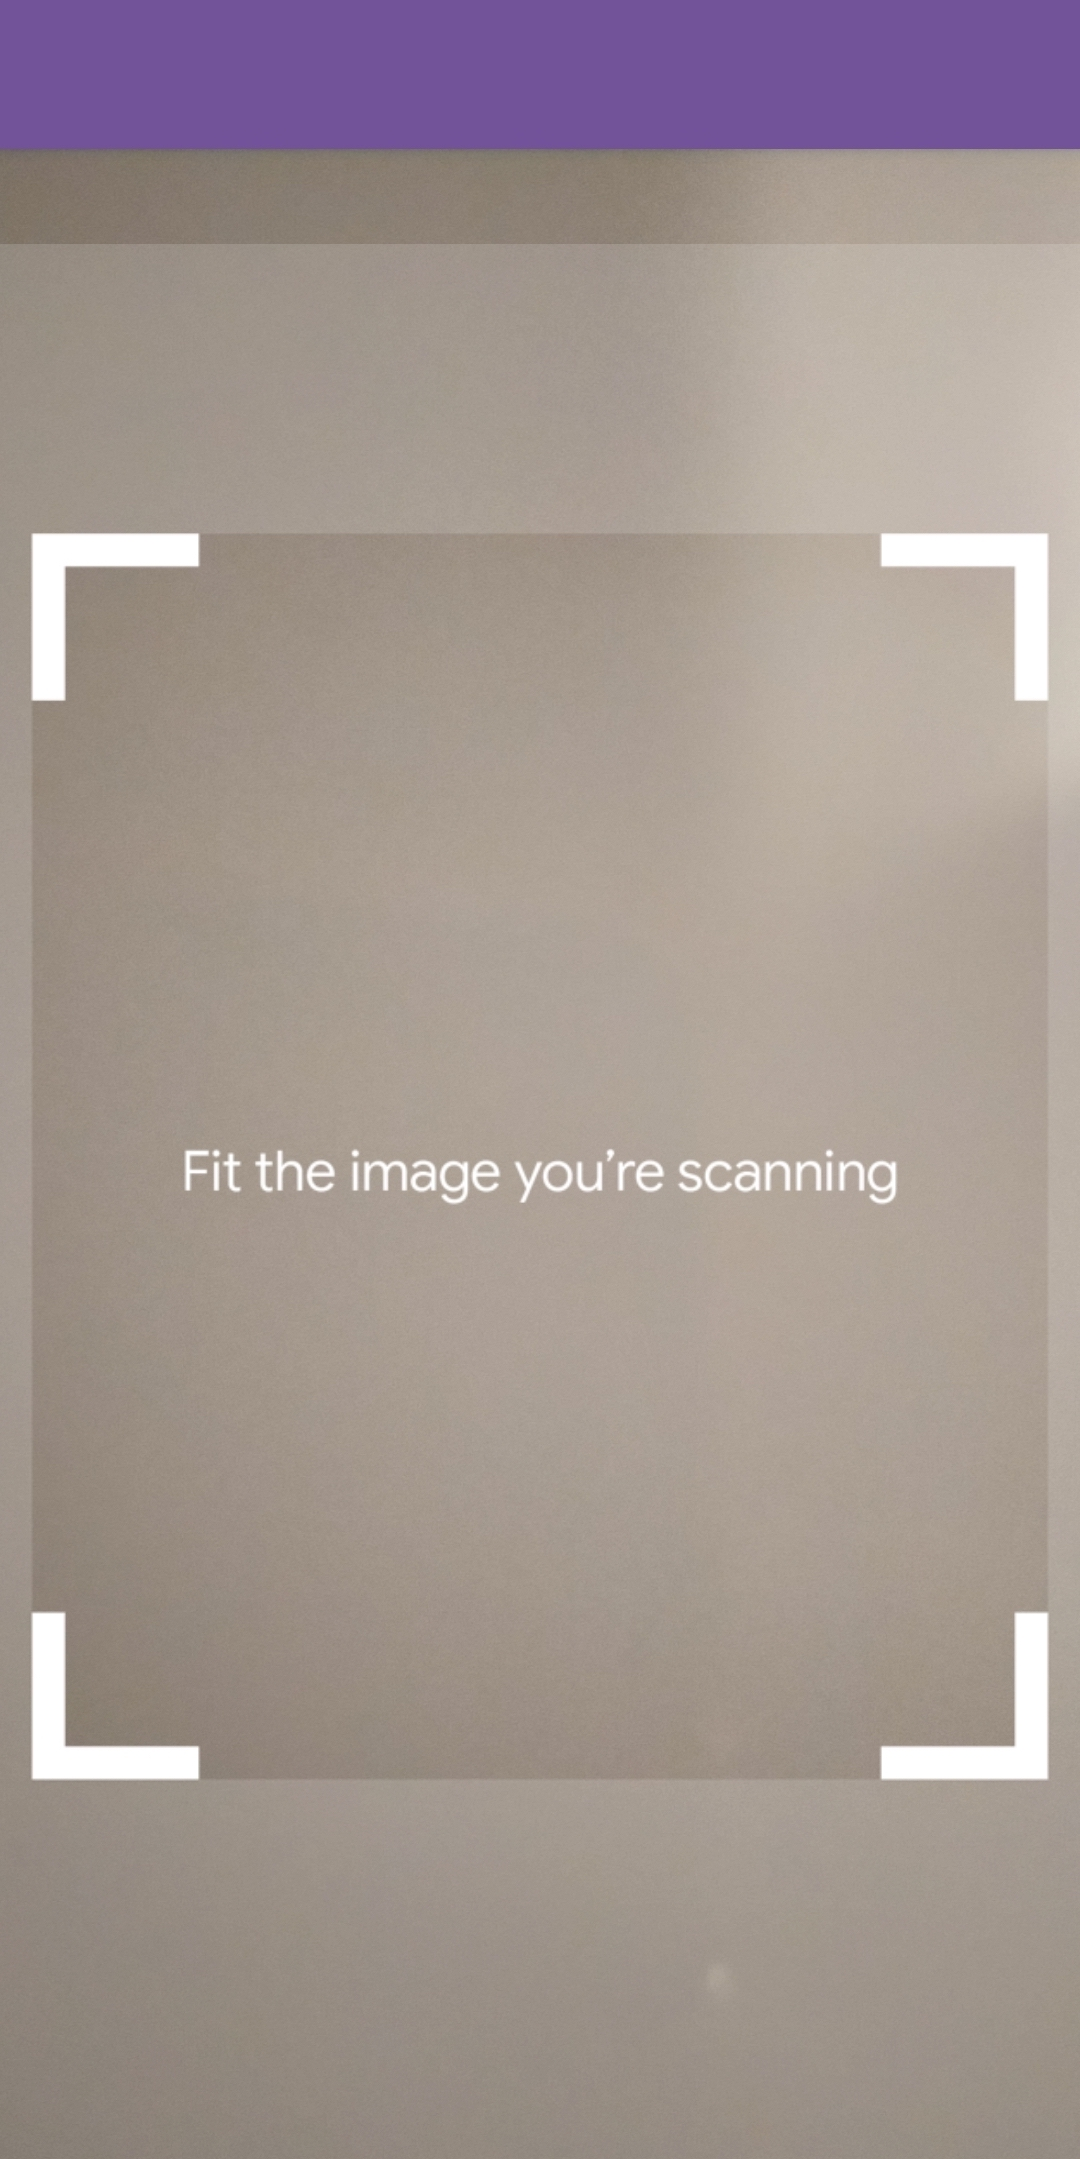
\includegraphics[width=7cm,height=7cm,keepaspectratio]{4Umsetzung/Bilder/image_tracking.jpg}
    \caption{Markererkennung der Applikation zum Start der Scan-Phase}
    \label{pic:image_tracking}
\end{figure}
\pagebreak 
\\
%\linebreak 
Des Weiteren beinhaltet das Assistenzsystem die eigentliche Scan-Phasen \acs{UI}, mit der die Umgebung aufgenommen wird und anhand dieser Daten 
der Nutzer die Objekte an von ihm definierte Stellen platzieren kann. Die Benutzeroberfläche hat ebenso ein schlichtes und überschaubares Layout, 
welches dem Anwender zugutekommt. 
\\ 
Hauptsächlich beinhaltet die \acs{GUI} ein Fragment, welches das Kamerabild in Echtzeit wiedergibt. Am oberen Ende des Bildschirms, bzw. der Abbildung 
(\ref{pic:scan}) befindet sich eine lilafarbene Fläche, die zur Anzeige von Informationen vorhanden ist und gleichzeitig als erweiterte Abgrenzung 
zur Topdown-Leiste dient. Am unteren Ende des Bildes befindet sich eine \textit{„Android-Gallery“}, die alle zu platzierenden Objekte beinhaltet. In 
der zugrundeliegenden Abbildung sind es zwei Platzhalter-Objekte, die bei Berührung des Bildes erstellt werden. Prinzipiell ist diese Gallery um 
beliebig viele Objekte erweiterbar. Diese Erweiterung erfolgt allerdings nicht dynamisch, sondern muss über manuelles Einfügen im Code stattfinden. 
%\\
%Wird während der laufenden Anwendung ein Objekt über dessen Button erstellt, wird der Nutzer unverzüglich auf eine weitere Seite %(\ref{pic:createObject}) 
%geleitet, um parallel zur Renderung des Objekts Informationen diesbezüglich der Datenbank hinzufügen zu können. Auf dieses Layout wird im weiteren Verlauf der 
%Ausarbeitung noch eingegangen. Vorwegzunehmen ist, dass die Informationen mit den Daten der virtuellen Position in der Datenbank persistiert werden.
%\\ 
%\linebreak 
%Damit der Scan-Vorgang gestartet wird
%Bevor der Scan-Vorgang startet, wird inmitten des Fragments ein Overlay angezeigt, welches eine Geste, bzw. Bewegung vorgibt. Imitiert der Nutzer 
%diese Bewegung, wird der Scan-Prozess anlaufen.
\\ 
\linebreak
Um weiterhin auf der Seite navigieren zu können, gibt es im rechten unteren Eck einen weiteren Button, welcher ebenso der Abbildung (\ref{pic:scan}) 
zu entnehmen ist. Diese Schaltfläche leitet den Nutzer weiter, bzw. wieder zurück zum Startmenü und beendet die Scan-Phase. 
\\ 
\linebreak
Damit der Nutzer über die in der Datenbank gespeicherten Informationen mehr Möglichkeiten besitzt, gibt es im linken oberen Eck der \acs{UI} eine zusätzliche 
Schaltfläche mit einem roten Kreuz versehen. Dadurch hat der Nutzer die Möglichkeit, alle vorhandenen, in der Datenbank persistierten Informationen zu 
löschen und den Scan-Vorgang erneut von der ursprünglichen Ausgangsposition zu beginnen. %Nachdem die Daten gelöscht werden, wird der Nutzer aufgefordert, den 
%Ursprungspunkt, den zu \textit{„trackenden“} Marker, abzuscannen und die Phase erneut zu beginnen. 
\\ 
Mit dieser Funktion verfügt der Nutzer über mehr Entscheidungsmöglichkeiten, bevor die Applikation komplett gelöscht und neu aufgespielt werden muss.
\begin{figure}[hbt!]
    \centering
    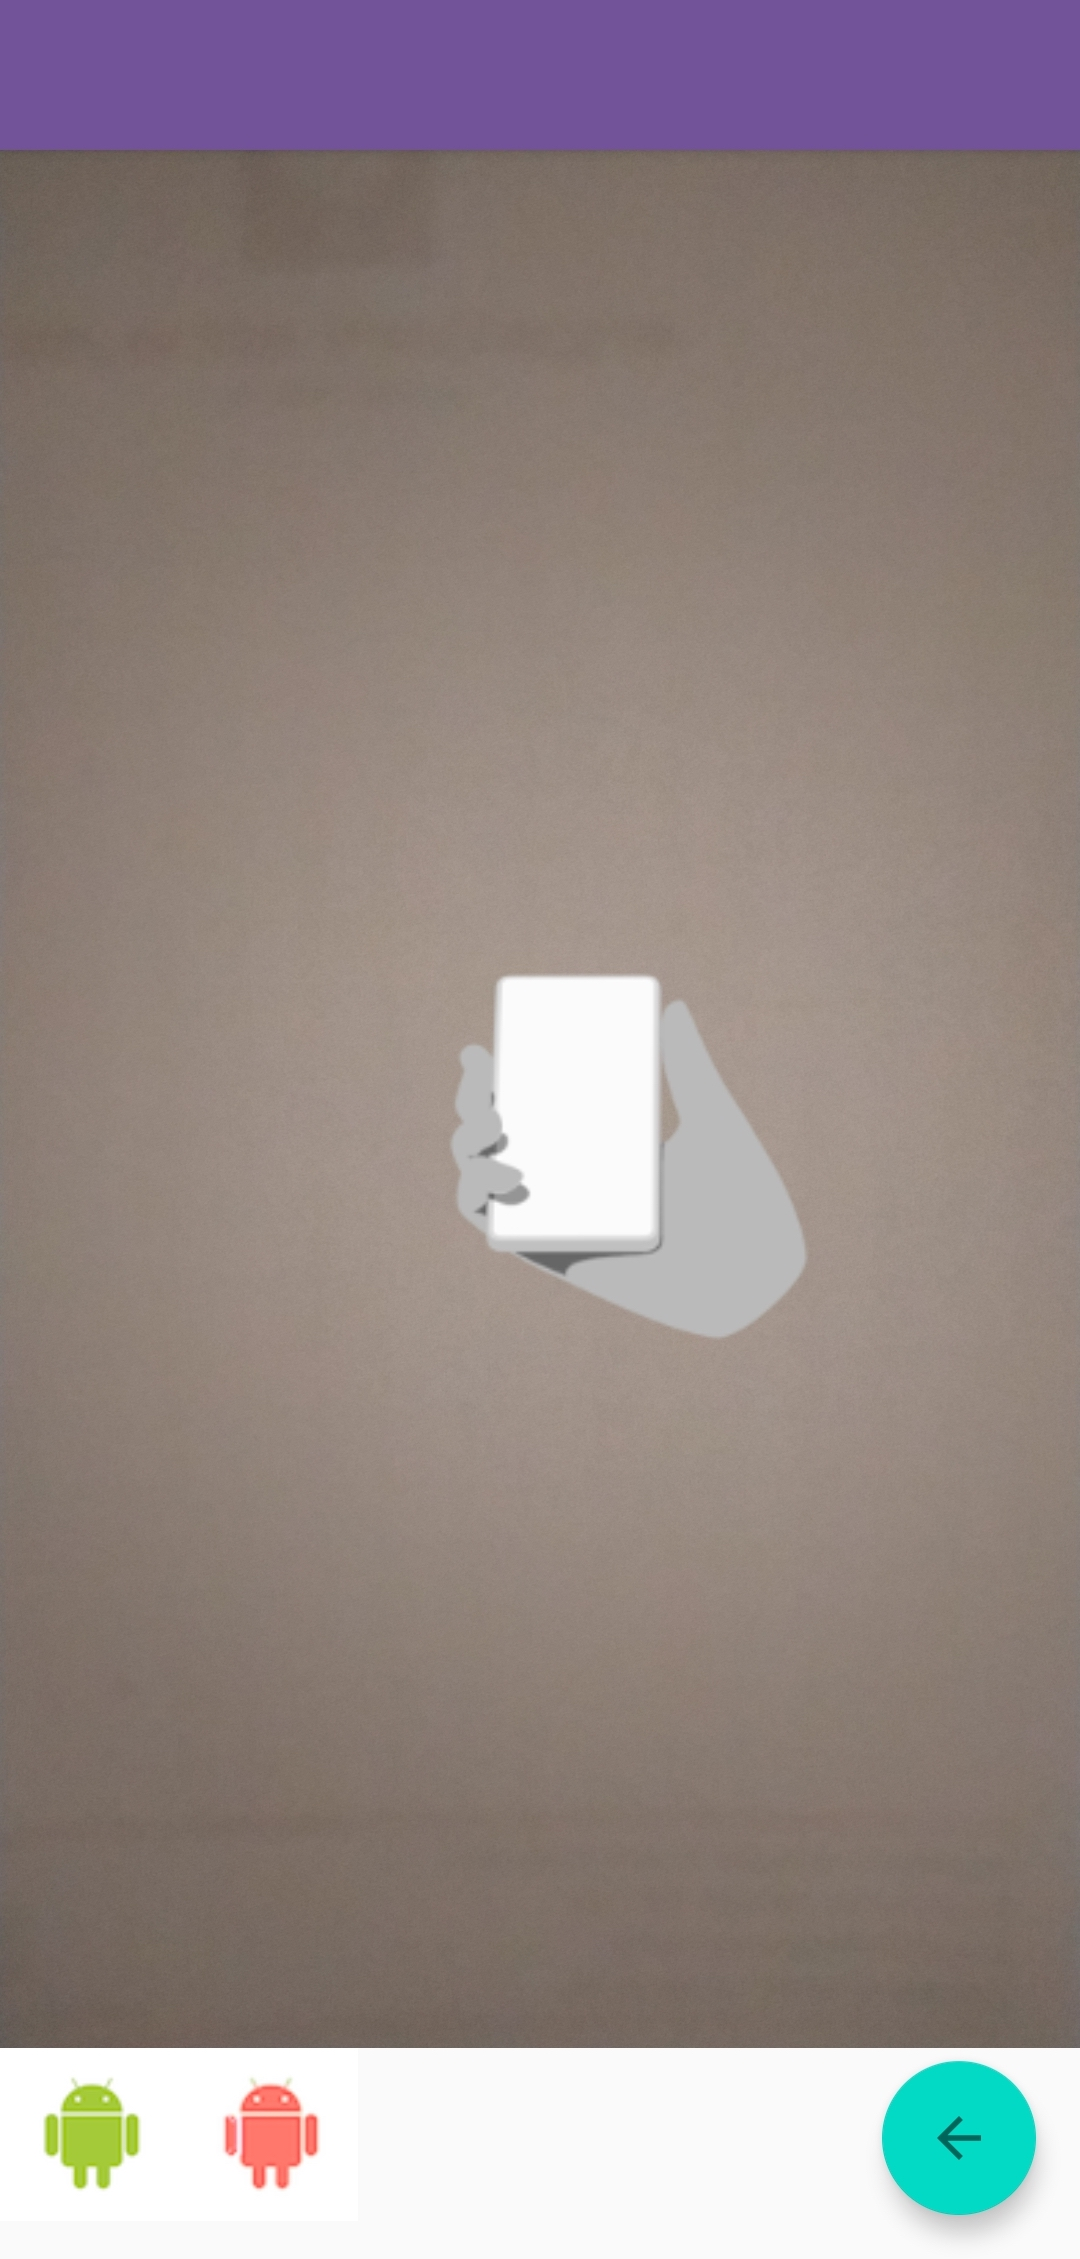
\includegraphics[width=7cm,height=7cm,keepaspectratio]{4Umsetzung/Bilder/scan-phase.jpg}
    \caption{Scan-Phase der Applikation}
    \label{pic:scan}
\end{figure}
\pagebreak
\\ %linebreak
Zu dem Zeitpunkt, wenn der Anwender ein Objekt erstellen und zusätzliche Informationen hinzufügen möchte, wird darauffolgend eine weitere \acs{UI} 
angezeigt. Bei dieser Ansicht ist vorgesehen, dass der Nutzer die zu dem erstellten Objekt dazugehörigen Informationen einträgt, sodass diese anschließend 
in die Datenbank aufgenommen werden können. Die Benutzeroberfläche verfügt über mehrere Text-Eingabefelder, die ein Großteil der Daten des Datenmodells 
abdecken. %In Abbildung (\ref{pic:createObject}) sind diese Felder zusehen. Dabei werden Informationen über den Objektnamen, -baujahr, -größe, sowie 
%-status von der Person, die das Assistenzsystem nutzt, gefordert. 
\\ 
Im Hintergrund werden ebenso die Daten der Position und Drehung des 
Objekts bereitgestellt.%Dies wird im Backend näher erläutert.%Über die Betätigung des \textit{„save“}-Buttons werden die Informationen lokal gespeichert und für die Eintragung in die Datenbank 
%vorgemerkt. Nachdem der Button bedient wurde, wird der Anwender auf die Oberfläche der Scan-Phase weitergeleitet, um bei Bedarf weitere Objekte zu 
%erstellen.  
%\begin{figure}[hbt!]
%    \centering
%    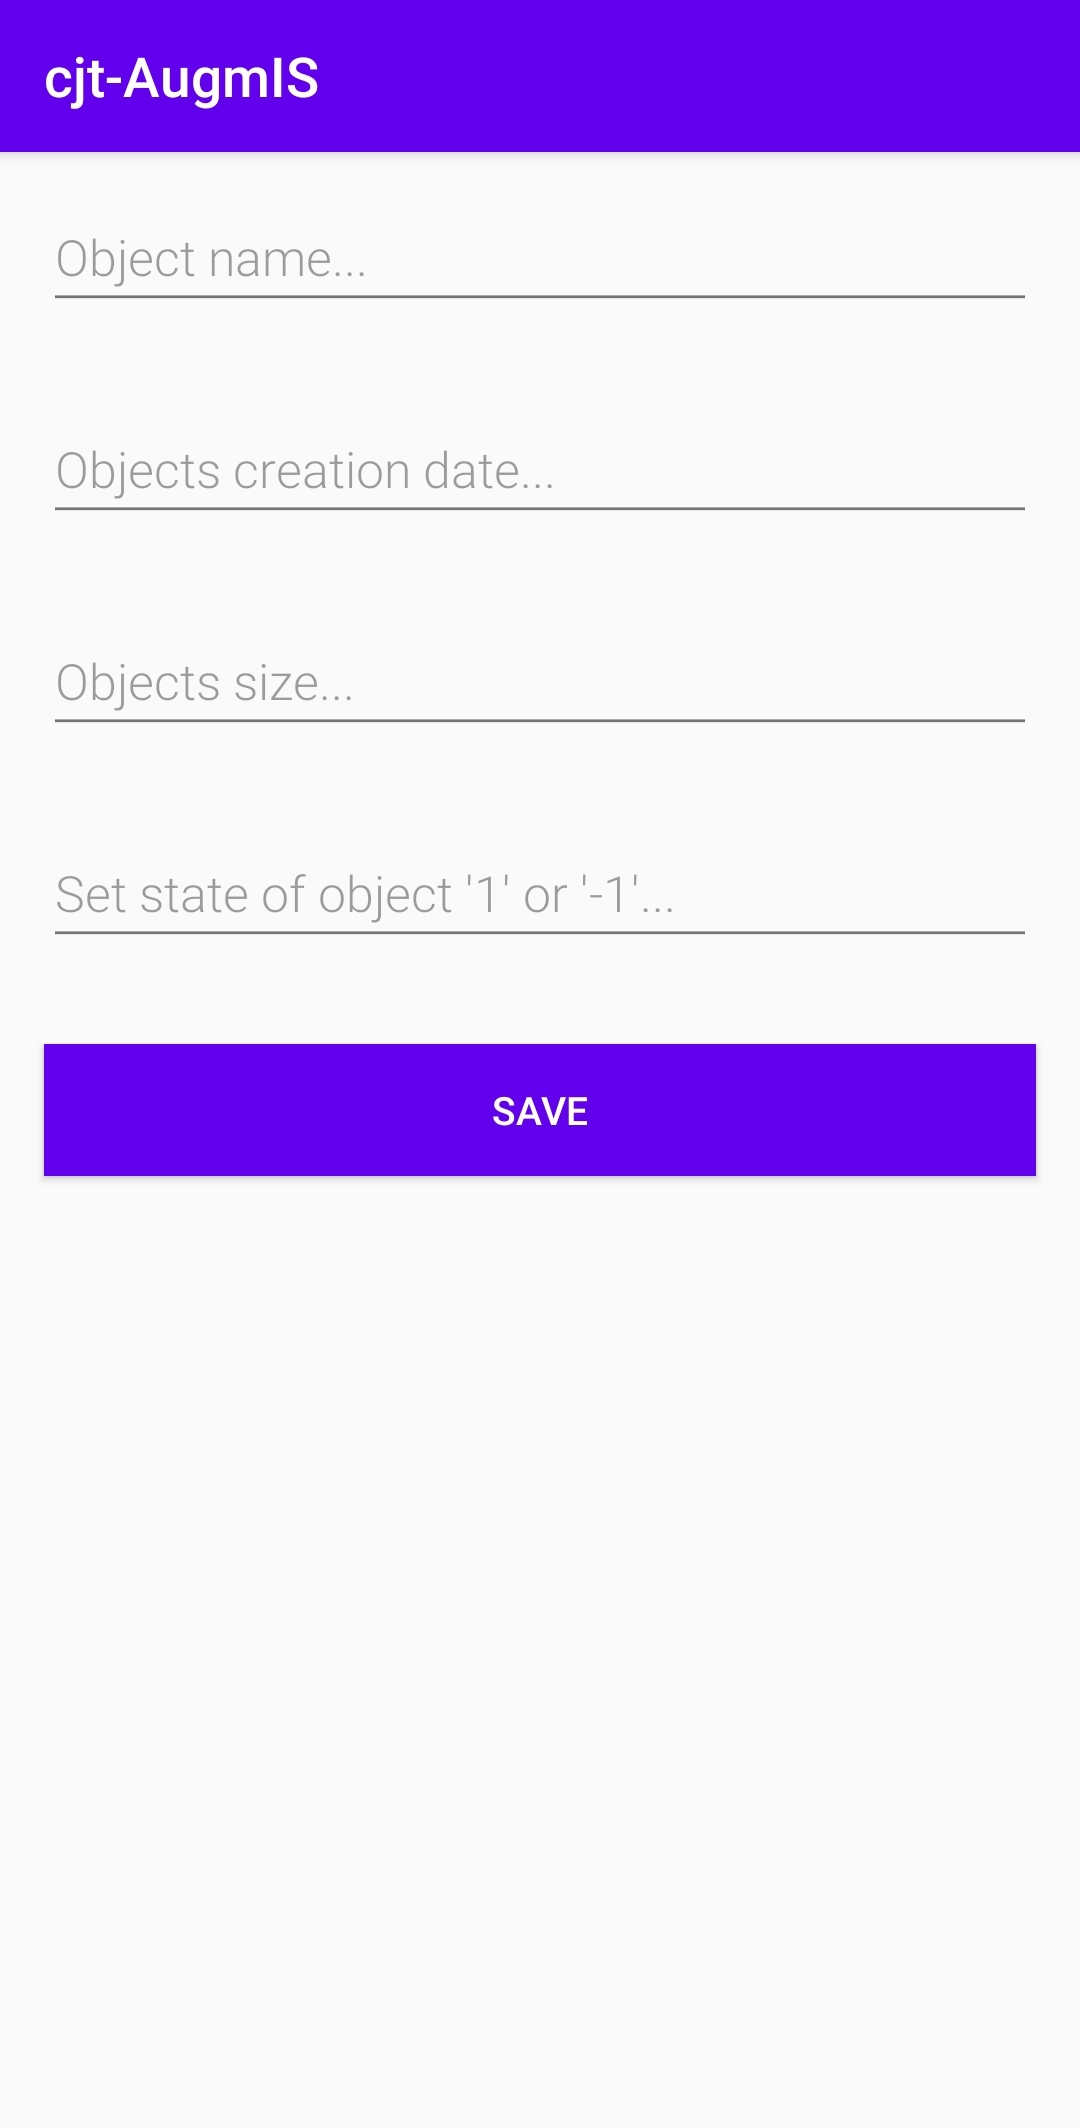
\includegraphics[width=7cm,height=7cm,keepaspectratio]{4Umsetzung/Bilder/objekt_info.jpg}
%    \caption{Erstellen eines neuen Objekts}
%    \label{pic:createObject}
%\end{figure}
%\pagebreak
%\\ 
%\linebreak
%Nachdem der Abschnitt der Frontend-Entwicklung vollends dargelegt wurde, geht es mit den Funktionen im Backend weiter. Darüber hinaus werden in diesem 
%Abschnitt auch die Lösungsansätze, sowie aufgetretene Probleme und deren Behebung genauestens aufgeführt und geschildert, damit der Nutzer mit der 
%aufgetretenen Problematik vertraut wird und die Entscheidungen und Lösungsfindungen nachvollziehen kann. 
\\ 
%\linebreak
Anhand des folgenden Programmablaufs wird der Ablauf der Scan-Phase veranschaulicht.
\begin{figure}[hbt!]
    \centering
    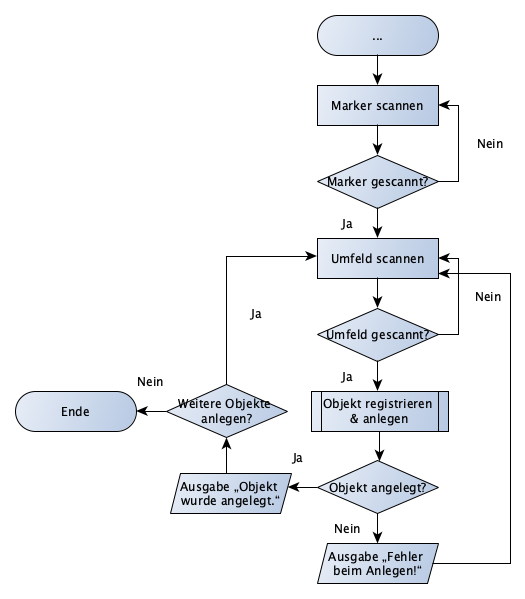
\includegraphics[width=10cm,height=9cm,keepaspectratio]{4Umsetzung/Bilder/scanPAP.png}
    \caption{Programmablaufplan der Scan-Phase}
    \label{pic:startmenu}
\end{figure}